\documentclass[12pt]{article}

% Computational Physics by M. Newman
% Setup file for exercises

% Packages
\usepackage{mathpazo}
\usepackage{amsmath}
\usepackage{graphicx}
\usepackage{calrsfs}
\usepackage{fancyvrb}

% Formatting
\setlength{\textwidth}{17.5cm}
\setlength{\textheight}{24.0cm}
\setlength{\evensidemargin}{2.5cm}
\setlength{\oddsidemargin}{-0.6cm}
\setlength{\topmargin}{-2.3cm}
\setlength{\textfloatsep}{0pt}
\setcounter{secnumdepth}{0}
\renewcommand{\baselinestretch}{1.06}

% Macros
\newcommand{\dd}{\mathrm{d}}
\newcommand{\ii}{\mathrm{i}}
\newcommand{\e}{\mathrm{e}}
\newcommand{\half}{\tfrac12}
\newcommand{\av}[1]{\langle#1\rangle}
\newcommand{\var}{\mathop\mathrm{var}}
\newcommand{\Ord}{\mathrm{O}}
\renewcommand{\Re}{\mathop\mathrm{Re}\nolimits}
\renewcommand{\Im}{\mathop\mathrm{Im}\nolimits}
\newcommand{\mat}{\mathbf}
\renewcommand{\vec}{\mathbf}
\newcommand{\defn}{\textit}
\newcommand{\exskip}{\nopagebreak\medskip\noindent}
\newcommand{\pmstrut}{\rule{0pt}{13pt}}

% Environments
\newcounter{chapter}
\setcounter{chapter}{2}
\newcounter{exercise}
\renewcommand{\theexercise}{\arabic{chapter}.\arabic{exercise}}
\newenvironment{exercises}{\vspace{2ex plus0.5ex minus0.5ex}
  \renewcommand{\labelenumi}{\alph{enumi})}}%
    {\par\vspace{1ex plus0.5ex minus0.5ex}}
\newcommand{\exercise}{\refstepcounter{exercise}%
  \par\vspace{4ex plus1ex minus1ex}%
  \noindent\textbf{Exercise \theexercise: }}

\DefineVerbatimEnvironment{code}{Verbatim}{xleftmargin=\parindent}

\setcounter{chapter}{2}

\begin{document}

\noindent {\LARGE\textsc{Computational Physics}}\par
\bigskip
\noindent {\large\textsc{Exercises for Chapter \arabic{chapter}}}\par
\noindent\hrulefill

%%%%%%%%%%%%%%%%%%%%%%%%%%%%%%%%%%%%%%%%%%%%%%%%%%%%%%%%%%%%%%%%%%%%%%
%%%                                                                %%%
%%%     COMPUTATIONAL PHYSICS, M. NEWMAN, CHAPTER 2, EXERCISES     %%%
%%%                                                                %%%
%%%%%%%%%%%%%%%%%%%%%%%%%%%%%%%%%%%%%%%%%%%%%%%%%%%%%%%%%%%%%%%%%%%%%%

\begin{exercises}

%%% Exercise 2.1 %%%

\exercise \textbf{Another ball dropped from a tower}

\exskip A ball is dropped from a tower of height~$h$ with initial velocity
zero.  Write a program that asks the user to enter the height in meters of
the tower and then calculates and prints the time the ball takes until it
hits the ground, ignoring air resistance.  Use your program to calculate
the time for a ball dropped from a $100\,$m high tower.


%%% Exercise 2.2 %%%

\exercise \textbf{Altitude of a satellite}

\exskip A satellite is to be launched into a circular orbit around the
Earth so that it orbits the planet once every~$T$ seconds.
\begin{enumerate}\setlength{\itemsep}{0pt}
\item Show that the altitude~$h$ above the Earth's surface that the
  satellite must have is
\begin{displaymath}
h = \biggl( {GMT^2\over4\pi^2} \biggr)^{1/3} - R,
\end{displaymath}
where
$G=6.67\times10^{-11}\,\textrm{m}^3\,\textrm{kg}^{-1}\,\textrm{s}^{-2}$ is
Newton's gravitational constant, $M=5.97\times10^{24}\,$kg is the mass of
the Earth, and $R=6371\,$km is its radius.
\item Write a program that asks the user to enter the desired value of~$T$
  and then calculates and prints out the correct altitude in meters.
\item Use your program to calculate the altitudes of satellites that orbit
  the Earth once a day (so-called ``geosynchronous'' orbit), once every 90
  minutes, and once every 45 minutes.  What do you conclude from the last
  of these calculations?
\item Technically a geosynchronous satellite is one that orbits the Earth
  once per \textit{sidereal day}, which is 23.93 hours, not 24 hours.  Why
  is this?  And how much difference will it make to the altitude of the
  satellite?
\end{enumerate}


%%% Exercise 2.3 %%%

\exercise Write a program to perform the inverse operation to that of
Example~2.2.  That is, ask the user for the Cartesian coordinates~$x,y$ of
a point in two-dimensional space, and calculate and print the corresponding
polar coordinates, with the angle~$\theta$ given in degrees.


%%% Exercise 2.4 %%%

\exercise A spaceship travels from Earth in a straight line at relativistic
speed~$v$ to another planet $x$ light years away.  Write a program to ask
the user for the value of~$x$ and the speed~$v$ as a fraction of the speed
of light~$c$, then print out the time in years that the spaceship takes to
reach its destination (a)~in the rest frame of an observer on Earth and
(b)~as perceived by a passenger on board the ship.  Use your program to
calculate the answers for a planet 10 light years away with $v=0.99c$.


%%% Exercise 2.5 %%%

\exercise \textbf{Quantum potential step}

\exskip A well-known quantum mechanics problem involves a particle of
mass~$m$ that encounters a one-dimensional potential step, like this:
\medskip
\begin{center}
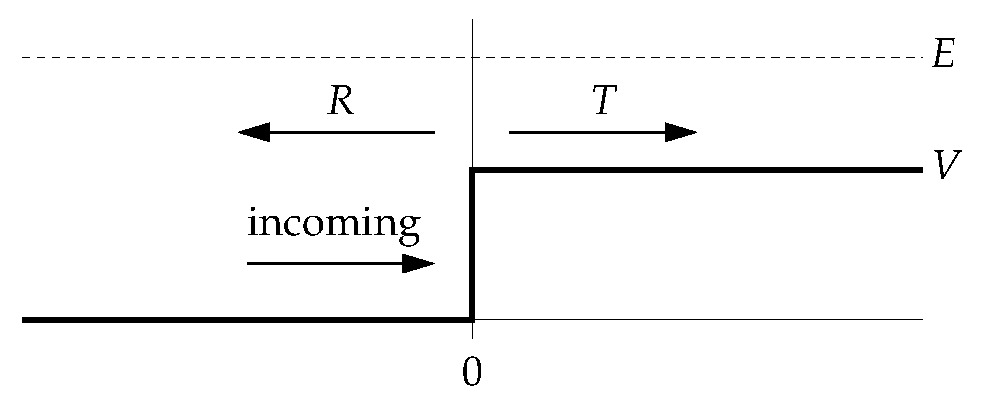
\includegraphics[width=9cm]{qstep.eps}
\end{center}
\smallskip The particle with initial kinetic energy~$E$ and
wavevector~$k_1=\sqrt{2mE}/\hbar$ enters from the left and encounters a
sudden jump in potential energy of height~$V$ at position~$x=0$.  By
solving the Schr\"odinger equation, one can show that when $E>V$ the
particle may either (a)~pass the step, in which case it has a lower kinetic
energy of $E-V$ on the other side and a correspondingly smaller wavevector
of $k_2=\sqrt{2m(E-V)}/\hbar$, or (b)~it may be reflected, keeping all of
its kinetic energy and an unchanged wavevector but moving in the opposite
direction.  The probabilities $T$ and $R$ for transmission and
reflection are given by
\begin{displaymath}
T = {4k_1k_2\over(k_1+k_2)^2}\,,\qquad
R = \biggl( {k_1-k_2\over k_1+k_2} \biggr)^2.
\end{displaymath}

Suppose we have a particle with mass equal to the electron mass
$m=9.11\times10^{-31}\,$kg and energy $10\,$eV encountering a potential
step of height~$9\,$eV.  Write a Python program to compute and print out
the transmission and reflection probabilities using the formulas above.


%%% Exercise 2.6 %%%

\exercise \textbf{Planetary orbits}

\nopagebreak\smallskip\noindent The orbit in space of one body
around another, such as a planet around the Sun, need not be
circular.  In general it takes the form of an ellipse, with the body
sometimes closer in and sometimes further out.  If you are given the
distance~$\ell_1$ of closest approach that a planet makes to the Sun, also
called its \defn{perihelion}, and its linear velocity~$v_1$ at
perihelion, then any other property of the orbit can be calculated
from these two as follows.
\begin{enumerate}\setlength{\itemsep}{0pt}
\item Kepler's second law tells us that the distance~$\ell_2$ and
  velocity~$v_2$ of the planet at its most distant point, or
  \defn{aphelion}, satisfy $\ell_2 v_2 = \ell_1 v_1$.  At the same
  time the total energy, kinetic plus gravitational, of a planet with
  velocity~$v$ and distance~$r$ from the Sun is given by
\begin{displaymath}
E = \half m v^2 - G {mM\over r},
\end{displaymath}
where $m$ is the planet's mass, $M=1.9891\times10^{30}\,$kg is the mass of
the Sun, and $G=6.6738\times10^{-11}\,\mathrm{m^3\,kg^{-1}\,s^{-2}}$ is
Newton's gravitational constant.  Given that energy must be conserved, show
that $v_2$ is the smaller root of the quadratic equation
\begin{displaymath}
v_2^2 - {2GM\over v_1\ell_1} v_2 - \biggl[ v_1^2 - {2GM\over\ell_1}
  \biggr] = 0.
\end{displaymath}
Once we have $v_2$ we can calculate $\ell_2$ using the relation $\ell_2 =
\ell_1 v_1/v_2$.
\item Given the values of $v_1$, $\ell_1$, and~$\ell_2$, other parameters
  of the orbit are given by simple formulas can that be derived from
  Kepler's laws and the fact that the orbit is an ellipse:
\begin{align*}
\textrm{Semi-major axis:} \qquad a &= \half(\ell_1+\ell_2), \\
\textrm{Semi-minor axis:} \qquad b &= \sqrt{\ell_1\ell_2}\,, \\
\textrm{Orbital period:} \hspace{1.80em}
  T &= {2\pi ab\over\ell_1 v_1}\,, \\
\textrm{Orbital eccentricity:} \qquad e &=
  {\ell_2-\ell_1\over\ell_2+\ell_1}.
\end{align*}
Write a program that asks the user to enter the distance to the Sun and
velocity at perihelion, then calculates and prints the quantities
$\ell_2$, $v_2$, $T$, and~$e$.
\item Test your program by having it calculate the properties of the orbits
  of the Earth (for which $\ell_1=1.4710\times10^{11}\,$m and
  $v_1=3.0287\times10^4\,\mathrm{m\,s^{-1}}$) and Halley's comet
  ($\ell_1=8.7830\times10^{10}\,$m and
  $v_1=5.4529\times10^4\,\mathrm{m\,s^{-1}}$).  Among other things, you
  should find that the orbital period of the Earth is one year and that of
  Halley's comet is about 76 years.
\end{enumerate}


%%% Exercise 2.7 %%%

\exercise \textbf{Catalan numbers}

\exskip The Catalan numbers~$C_n$ are a sequence of integers 1, 1, 2, 5,
14, 42, 132\dots that play an important role in quantum mechanics and the
theory of disordered systems.  (They were central to Eugene Wigner's proof
of the so-called semicircle law.)  They are given~by
\begin{displaymath}
C_0 = 1,\qquad C_{n+1} = {4n+2\over n+2}\,C_n.
\end{displaymath}
Write a program that prints in increasing order all Catalan numbers less
than or equal to one billion.


%%% Exercise 2.8 %%%

\exercise Suppose arrays \verb|a| and \verb|b| are defined as follows:
\begin{code}
from numpy import array
a = array([1,2,3,4],int)
b = array([2,4,6,8],int)
\end{code}
What will the computer print upon executing the following lines?  (Try to
work out the answer before trying it on the computer.)
\begin{enumerate}\setlength{\itemsep}{0pt}\setlength{\parskip}{0pt}
\item \verb|print(b/a+1)|
\item \verb|print(b/(a+1))|
\item \verb|print(1/a)|
\end{enumerate}


%%% Exercise 2.9 %%%

\exercise \textbf{The Madelung constant}

\exskip In condensed matter physics the Madelung constant gives the total
electric potential felt by an atom in a solid.  It depends on the charges
on the other atoms nearby and their locations.  Consider for instance solid
sodium chloride---table salt.  The sodium chloride crystal has atoms
arranged on a cubic lattice, but with alternating sodium and chlorine
atoms, the sodium ones having a single positive charge $+e$ and the
chlorine ones a single negative charge~$-e$, where $e$ is the charge on the
electron.  If we label each position on the lattice by three integer
coordinates $(i,j,k)$, then the sodium atoms fall at positions where
$i+j+k$ is even, and the chlorine atoms at positions where $i+j+k$ is odd.

Consider a sodium atom at the origin, $i=j=k=0$, and let us calculate the
Madelung constant.  If the spacing of atoms on the lattice is~$a$, then the
distance from the origin to the atom at position $(i,j,k)$ is
\begin{displaymath}
\sqrt{(ia)^2 + (ja)^2 + (ka)^2} = a \sqrt{i^2+j^2+k^2},
\end{displaymath}
and the potential at the origin created by such an atom is
\begin{displaymath}
V(i,j,k) = \pm {e\over4\pi\epsilon_0 a\sqrt{i^2+j^2+k^2}},
\end{displaymath}
with $\epsilon_0$ being the permittivity of the vacuum and the sign of the
expression depending on whether $i+j+k$ is even or odd.  The total
potential felt by the sodium atom is then the sum of this quantity over all
other atoms.  Let us assume a cubic box around the sodium at the origin,
with $L$ atoms in all directions.  Then
\begin{displaymath}
V_\textrm{total} = \sum_{\substack{i,j,k=-L\\ \textrm{not }i=j=k=0}}^L
                   \hspace{-0.5em} V(i,j,k)
                 = {e\over4\pi\epsilon_0 a}\,M,
\end{displaymath}
where $M$ is the Madelung constant, at least approximately---technically
the Madelung constant is the value of~$M$ when $L\to\infty$, but one can
get a good approximation just by using a large value of~$L$.

Write a program to calculate and print the Madelung constant for sodium
chloride.  Use as large a value of $L$ as you can, while still having your
program run in reasonable time---say in a minute or less.


%%% Exercise 2.10 %%%

\exercise \textbf{The semi-empirical mass formula}

\exskip In nuclear physics, the semi-empirical mass formula is a formula
for calculating the approximate nuclear binding energy~$B$ of an atomic
nucleus with atomic number~$Z$ and mass number~$A$:
\begin{displaymath}
B = a_1 A - a_2 A^{2/3} - a_3 {Z^2\over A^{1/3}}
    - a_4 {(A - 2Z)^2\over A} + {a_5\over A^{1/2}}\,,
\end{displaymath}
where, in units of millions of electron volts, the constants are
$a_1=15.67$, $a_2=17.23$, $a_3=0.75$, $a_4=93.2$, and
\begin{displaymath}
a_5 = \left\lbrace\begin{array}{ll}
      0     &\quad\mbox{if $A$ is odd,} \\
      12.0  &\quad\mbox{if $A$ and $Z$ are both even,} \\
      -12.0 &\quad\mbox{if $A$ is even and $Z$ is odd.}
      \end{array}\right.
\end{displaymath}
\begin{enumerate}\setlength{\itemsep}{0pt}
\item Write a program that takes as its input the values of $A$ and $Z$,
  and prints out the binding energy for the corresponding atom.  Use your
  program to find the binding energy of an atom with $A=58$ and $Z=28$.
  (Hint: The correct answer is around $490\,$MeV.)
\item Modify your program to print out not the total binding energy~$B$,
  but the binding energy per nucleon, which is~$B/A$.
\item Now modify your program so that it takes as input just a single value
  of the atomic number~$Z$ and then goes through all values of~$A$ from
  $A=Z$ to $A=3Z$, to find the one that has the largest binding energy per
  nucleon.  This is the most stable nucleus with the given atomic number.
  Have your program print out the value of~$A$ for this most stable nucleus
  and the value of the binding energy per nucleon.
\item Modify your program again so that, instead of taking $Z$ as input, it
  runs through all values of $Z$ from 1 to 100 and prints out the most
  stable value of $A$ for each one.  At what value of~$Z$ does the maximum
  binding energy per nucleon occur?  (The true answer, in real life, is
  $Z=28$, which is nickel.  You should find that the semi-empirical mass
  formula gets the answer roughly right, but not exactly.)
\end{enumerate}


%%% Exercise 2.11 %%%

\exercise \textbf{Binomial coefficients}

\exskip The binomial coefficient ${n\choose k}$ is an integer equal to
\begin{displaymath}
{n\choose k} = {n!\over k!(n-k)!}
  = {n\times(n-1)\times(n-2)\times\ldots\times(n-k+1)\over
     1\times2\times\ldots\times k}
\end{displaymath}
when $k\ge1$, or ${n\choose0}=1$ when $k=0$.
\begin{enumerate}\setlength{\itemsep}{0pt}
\item Using this form for the binomial coefficient, write a user-defined
  function \verb|binomial(n,k)| that calculates the binomial coefficient
  for given $n$ and~$k$.  Make sure your function returns the answer in the
  form of an integer (not a float) and gives the correct value of~1 for the
  case where $k=0$.
\item Using your function write a program to print out the first 20 lines
  of ``Pascal's triangle.''  The $n$th line of Pascal's triangle contains
  $n+1$ numbers, which are the coefficients ${n\choose 0}$, ${n\choose1}$,
  and so on up to ${n\choose n}$.  Thus the first few lines are
\begin{flushleft}
1 1 \\
1 2 1 \\
1 3 3 1 \\
1 4 6 4 1
\end{flushleft}
\item The probability that an unbiased coin, tossed $n$ times, will come up
  heads $k$ times is ${n\choose k}/2^n$.  Write a program to calculate
  (a)~the total probability that a coin tossed 100 times comes up heads
  exactly 60 times, and (b)~the probability that it comes up heads 60 or
  more times.
\end{enumerate}


%%% Exercise 2.12 %%%

\exercise \textbf{Prime numbers}

\exskip The program in Example~2.8 is not a very efficient way of
calculating prime numbers: it checks each number to see if it is divisible
by any number less than it.  We can develop a much faster program for prime
numbers by making use of the following observations:
\begin{enumerate}\setlength{\itemsep}{0pt}
\item A number~$n$ is prime if it has no prime factors less than~$n$.
  Hence we only need to check if it is divisible by other primes.
\item If a number~$n$ is non-prime, having a factor~$r$, then $n=rs$, where
  $s$ is also a factor.  If $r\ge\sqrt{n}$ then $n = rs \ge \sqrt{n}s$,
  which implies that $s\le\sqrt{n}$.  In other words, any non-prime must
  have factors, and hence also prime factors, less than or equal
  to~$\sqrt{n}$.  Thus to determine if a number is prime we have to check
  its prime factors only up to and including~$\sqrt{n}$---if there are none
  then the number is prime.
\item If we find even a single prime factor less than~$\sqrt{n}$ then we
  know that the number is non-prime, and hence there is no need to check
  any further---we can abandon this number and move on to something else.
\end{enumerate}
Write a Python program that finds all the primes up to ten thousand.
Create a list to store the primes, which starts out with just the one prime
number~2 in it.  Then for each number~$n$ from 3 to $10\,000$ check whether
the number is divisible by any of the primes in the list up to and
including~$\sqrt{n}$.  As soon as you find a single prime factor you can
stop checking the rest of them---you know~$n$ is not a prime.  If you find
no prime factors $\sqrt{n}$ or less then $n$ is prime and you should add it
to the list.  You can print out the list all in one go at the end of the
program, or you can print out the individual numbers as you find them.


%%% Exercise 2.13 %%%

\exercise \textbf{Recursion}

\exskip A useful feature of user-defined functions is \defn{recursion}, the
ability of a function to call itself.  For example, consider the following
definition of the factorial~$n!$ of a positive integer~$n$:
\begin{displaymath}
n! = \biggl\lbrace\begin{array}{ll}
  1 & \qquad\mbox{if $n=1$,} \\
  n\times(n-1)! & \qquad\mbox{if $n>1$.}
\end{array}
\end{displaymath}
This constitutes a complete definition of the factorial which allows us to
calculate the value of $n!$ for any positive integer.  We can employ this
definition directly to create a Python function for factorials, like this:
\begin{code}
def factorial(n):
    if n==1:
        return 1
    else:
        return n*factorial(n-1)
\end{code}
Note how, if $n$ is not equal to~1, the function calls itself to calculate
the factorial of $n-1$.  This is recursion.  If we now say
``\verb|print(factorial(5))|'' the computer will correctly print the
answer~120.
\begin{enumerate}\setlength{\itemsep}{0pt}
\item We encountered the Catalan numbers~$C_n$ previously in Exercise~2.7
  on page~46.  With just a little rearrangement, the definition given there
  can be rewritten in the form
\begin{displaymath}
C_n = \left\lbrace\begin{array}{ll}
  \rule[-9pt]{0pt}{10pt}1 & \qquad\mbox{if $n=0$,} \\
  \dfrac{4n-2}{n+1}\,C_{n-1} & \qquad\mbox{if $n>0$.}
\end{array}\right.
\end{displaymath}
Write a Python function, using recursion, that calculates~$C_n$.  Use your
function to calculate and print~$C_{100}$.
\item Euclid showed that the greatest common divisor~$g(m,n)$ of two
  nonnegative integers $m$ and $n$ satisfies
\begin{displaymath}
g(m,n) = \biggl\lbrace\begin{array}{ll}
  m & \qquad\mbox{if $n=0$,} \\
  g(n,m\>\textrm{mod}\>n) & \qquad\mbox{if $n>0$.}
\end{array}
\end{displaymath}
Write a Python function \verb|g(m,n)| that employs recursion to calculate
the greatest common divisor of $m$ and $n$ using this formula.  Use your
function to calculate and print the greatest common divisor of 108 and~192.
\end{enumerate}
Comparing the calculation of the Catalan numbers in part~(a) above with
that of Exercise~2.7, we see that it's possible to do the calculation two
ways, either directly or using recursion.  In most cases, if a quantity can
be calculated \emph{without} recursion, then it will be faster to do so,
and we normally recommend taking this route if possible.  There are some
calculations, however, that are essentially impossible (or at least much
more difficult) without recursion.  We will see some examples later in this
book.

\end{exercises}

\end{document}
